\chapter{Etude  d\'{e}cisionnelle}


ajouter du talend a la realisation

ici juste decrire
\subsection{Axes de l'Etude d\'{e}cisionnelle }

\bigskip
Notre \'{e}tude d\'{e}cisionnelle portera sur :

\begin{itemize}
\item{Le co\^{u}t total de chaque projet}
\item{Le co\^{u}t total des projets pour chaque client}
\item{Le co\^{u}t  total par catégrie des projets }
\item{La dur\'{e}e totale de chaque projet}
\end{itemize}





\subsection{Tests sur power bi }
captures


Nous avons besoin d'ajuster quelques champs pour etre ad\'{e}quates \`{a} etre
exploit\'{e}es .
Par exemple dans la table membre on trouve \guillemotleft{} firstname \guillemotright{} et \guillemotleft{} lastname \guillemotright{}
Et on doit les concat\'{e}ner pour dans une hi\'{e}rarchie pour avoir des rapports
lisibles \`{a} propos des membres .



\FloatBarrier
\begin{figure}[H]
\center
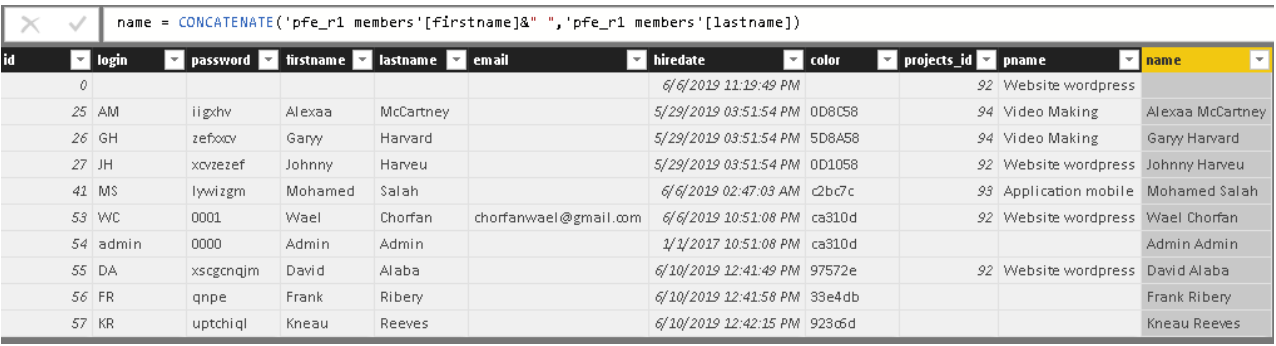
\includegraphics[width=14cm,height=5cm]{./figures/pb1.png}
\caption{Ajustement des noms.}
\end{figure}
\FloatBarrier


\bigskip
\bigskip

\FloatBarrier
\begin{figure}[H]
\center
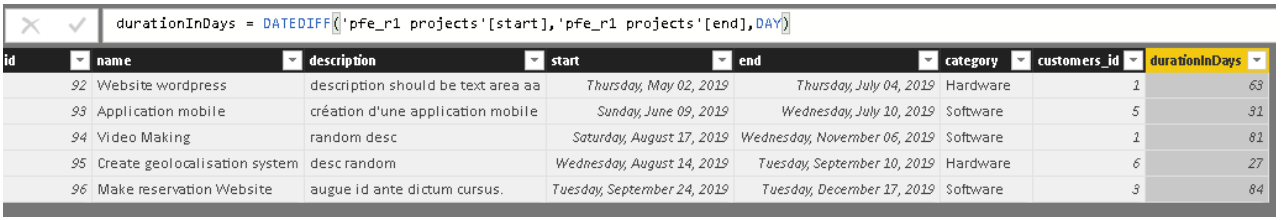
\includegraphics[width=14cm,height=3cm]{./figures/pb2.png}
\caption{Ajustement de la dur\'{e}e totale des projets.}
\end{figure}
\FloatBarrier

\newpage
\subsubsection{Reporting }
Pour tester les rapports et la validit\'{e} des donn\'{e}es , nous avons utilis\'{e} l'outil
Power BI pour nous donner une impression sur les rapports qu'on doit
int\'{e}grer \`{a} notre application afin de les visulaiser.

\bigskip
Pour ce fait on a cr\'{e}e les rapports correspontdants \`{a} l'\'{e}tude d\'{e}cisionnelle :
Les deux axes importants de l'\'{e}tude sont les couts et la dur\'{e}e :



\begin{itemize}

\item{ \textbf{Les  co\^{u}ts}  }

\FloatBarrier
\begin{figure}[H]
\center
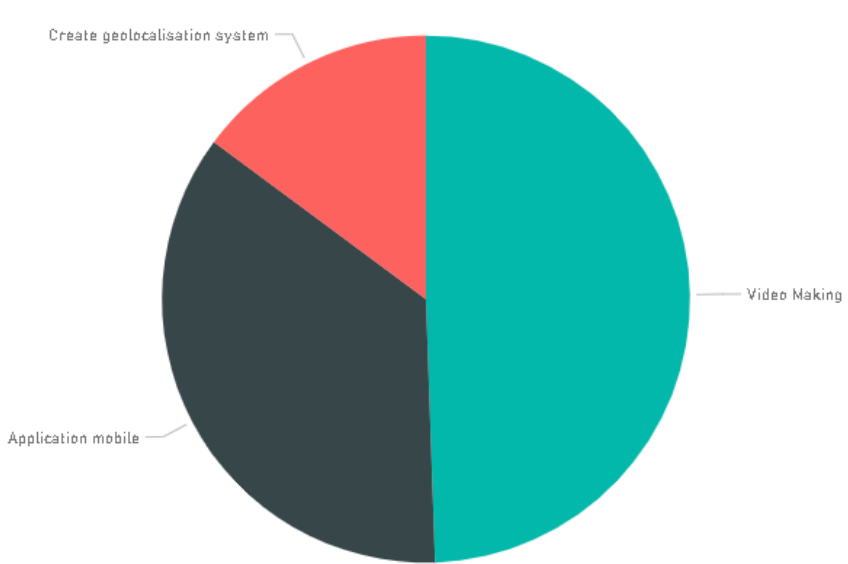
\includegraphics[width=10cm,height=10cm]{./figures/rpb1.png}
\caption{Co\^{u}t total par projet.}

\end{figure}
\FloatBarrier

\FloatBarrier
\begin{figure}[H]
\center
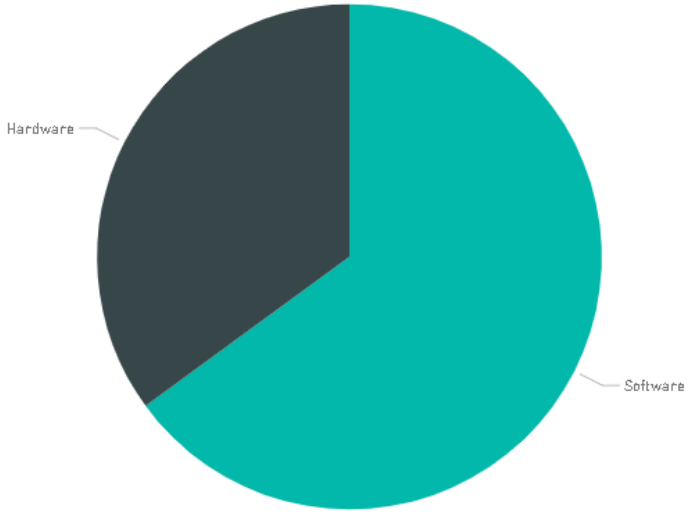
\includegraphics[width=10cm,height=10cm]{./figures/rpb2.png}
\caption{Co\^{u}t total par catégorie de projet.}

\end{figure}
\FloatBarrier

\FloatBarrier
\begin{figure}[H]
\center
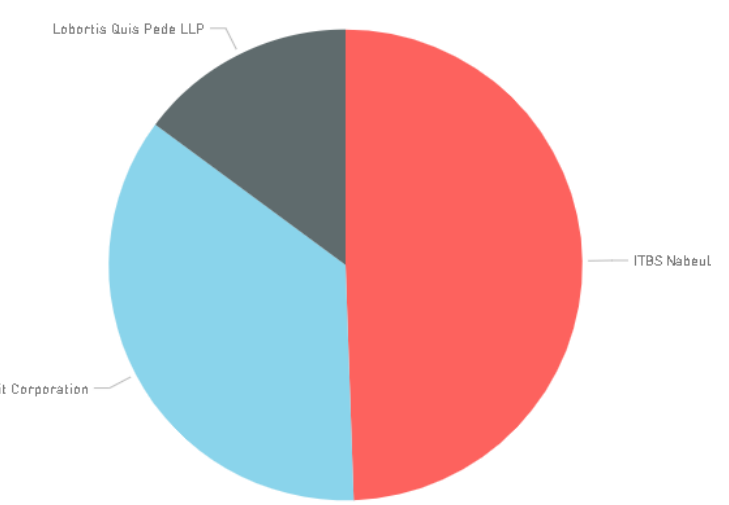
\includegraphics[width=10cm,height=10cm]{./figures/rpb3.png}
\caption{Co\^{u}t total par client.}

\end{figure}
\FloatBarrier

\FloatBarrier
\begin{figure}[H]
\center
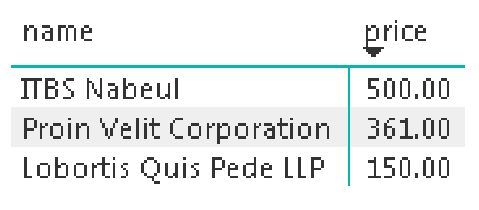
\includegraphics[width=8cm,height=5cm]{./figures/rpb31.png}
\caption{Co\^{u}t total par client en chiffres.}

\end{figure}
\FloatBarrier



\newpage

\item{ \textbf{La dur\'{e}e}  }
\FloatBarrier
\begin{figure}[H]
\center
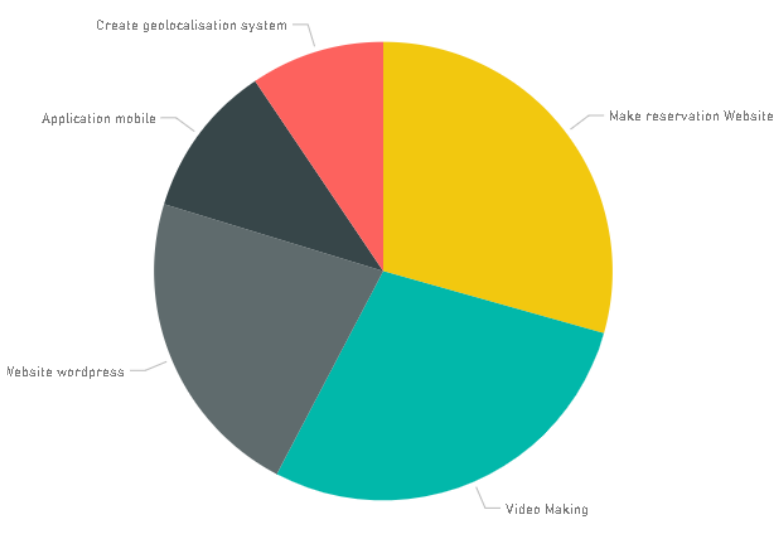
\includegraphics[width=10cm,height=10cm]{./figures/rpb4.png}
\caption{Dur\'{e}e total par projet (en jours).1}

\end{figure}
\FloatBarrier

\FloatBarrier
\begin{figure}[H]
\center
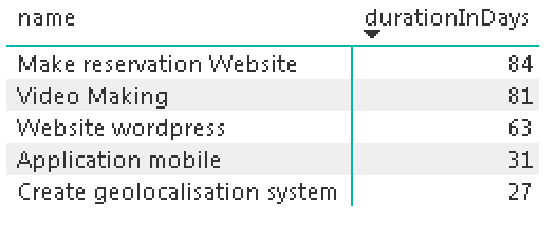
\includegraphics[width=8cm,height=5cm]{./figures/rpb42.png}
\caption{Dur\'{e}e total par projet (en jours).2}

\end{figure}
\FloatBarrier


\end{itemize}



\subsection{ETL}

Talend how
base 1 vers base 2
